\chapter{Markov Process}

Prior to any theory of Markov process, we need to at least introduce some general terms of stochastic processes that are necessary to undestand the context in following chapters and in the practical applications.

In following sections we consider probability space $\probSpace$.


%%%%%%%%%%%%%%%%%%%%%%%%%%%%%%%%%%%%%%%%%%%%%%%%%%%%%%%%%%%%%%%%%%%%%%%%%%%%%%%%%%%%%%%
%%%%%%%%%%%%%%%%%%%%%%%%%%%%%%%%%%%%%%%%%%%%%%%%%%%%%%%%%%%%%%%%%%%%%%%%%%%%%%%%%%%%%%%
\section{Stochastic Process}
\label{chap:basics}

There are several books about stochastic processes and most of the theory can be found in books about probability in general. In this section, we mention some of the sources while referring to the proofs of propositions that does not have to be proven in this thesis.

Let us begin with the definition of a stochastic process.

\begin{definition}\label{stochProc}
	Let $\procX$ be a family of random variables defined on probability space $\probSpace$. Then we call $\m{X}$ a \emph{stochastic process}.
\end{definition}

Kolmogorov consistency theorem states about necessary condition for existence of stochastic process.

\begin{theorem}[Daniell-Kolmogorov]\label{Kolmogorov}
  Let $\{\pr_{t_1, \ldots ,t_n}: 0\leq t_1\leq  \ldots  \leq t_n <\infty, n\in\mathbb{N} \}$ be a system of finite-dimensional distributions for which holds
	\begin{multline*}
		\pr_{t_1, \ldots t_{k-1},t_{k+1}, \ldots ,t_n}(B_1\times  \ldots \times B_{k-1} \times B_{k+1} \times  \ldots  \times B_n)\\
		= \pr_{t_1, \ldots ,t_n}(B_1\times \ldots \times B_{k-1} \times \mathbb{R} \times B_{k+1} \times  \ldots  \times B_n)
	\end{multline*}
	for all $n\in\mathbb{N}$, $1 \geq k \geq n$, $0\leq t_1\leq  \ldots  \leq t_n <\infty$ a $B_i \in \mathcal{B}$. Then there exists a stochastic process, whose finite-dimensional distributions are given by this system.
\end{theorem}

\begin{proof}
	For example in \cite{Stepan87}, Theorem I.10.3.
\end{proof}

Following definitions will become useful when studying Markov processes. We state them just to introduce the terminology. We will not discuss their properties and relations too much in detail. The reader can find details in any introductory book of stochastic processes.

\begin{definition}\label{stochEquiv}
	Let $\procX$ and $\proc{Y}$ are stochastic processes defined on the same probability space $\probSpace$. If $\pr [X_t = Y_t] = 1$ for all $t \geq 0$ then we say that $\m{X}$ and $\m{Y}$ are \emph{stochastically equivalent}.
\end{definition}

\begin{definition}\label{stochCont}
	A stochastic process $\procX$ is called \emph{stochastically continuous at point} $t \geq 0$ if for any $\epsilon > 0$
	\[
		\lim_{s \to t} \pr (\vert X_s - X_t \vert > \epsilon ) = 0.
	\]
	If $\m{X}$ is stochastically continuous at every point $t \geq 0$ then we say that it is \emph{stochastically continuous}.
\end{definition}

\begin{definition}\label{separProc}
	Let $\procX$ be a stochastic process defined on probability space $\probSpace$, $D \subset \Rplus$ be a countable dense set and $\Lambda \subset \Omega$ be a zero-probability event. If for any close set $C \subset \R$ and any open interval $J \subset \Rplus$ holds
	\[
		\{ \omega: X_t(\omega) \in C, t \in J \cap D \}
		\backslash
		\{ \omega: X_t(\omega) \in C, t \in J \}
		\subset \Lambda
	\]
	then we say that $\m{X}$ is \emph{separable}.
\end{definition}

\begin{definition}\label{measurProc}
	We will call $\procX$ a \emph{measurable stochastic process} if mapping $(\omega, t) \to X_t(\omega)$ is measurable with respect to product $\sigma$-algebra $\mathcal{A} \otimes \mathcal{B}(\Rplus)$.
\end{definition}

We state two theorems providing relations between the two of the defined terms that are necessary for this thesis. Both the propositions are taken from \cite{Doob90} and are left without any proof. The reader can find one in said literature.

\begin{proposition}\label{version}
	Let $\procX$ be a stochastically continuous process. Then there exists separable and measurable stochastic process that is equivalent to process $\m{X}$.
\end{proposition}

By previous proposition we can consider only process that is separable and measurable when we are given distribution of a stochastically continuous process.

\begin{lemma}\label{separDoob}
	Let $\procX$ be a stochastically continuous and separable process and $\{D_n = t_0^{(n)} < \ldots  < t_n^{(n), n \in \N} \}$ be a sequence of subdivisions of an interval $[s, s+h]$ for which $\| D_n \| \to 0$ as $n \to \infty$. Then
	\[
		\lim_{n \to \infty} \pr (X_{t_0^{(n)}} = i, \ldots , X_{t_n^{(n)}} = i)
		= \pr (X_t = i, s \leq t \leq s+h)
	\]
\end{lemma}

Finally, let us introduce the idea of time of random event. This concept is a basis for Markov process with continuous time and its transformation into discrete time.

\begin{definition}\label{markovTime}
	Let $\proc{X}$ be a stochastic process and $\tau : \Omega \to [0,\infty]$ be a measurable function. If $[\tau \leq t] \in \mathcal{F}_t \equiv \sigma (X_s, s \leq t)$ then we call $\tau$ a \emph{Markov time} of process $\m{X}$.
	
	Family of $\sigma$-algebras $\mathcal{F} = \{ \mathcal{F}_t, t \geq 0} \}$ is called a \emph{natural filtration} of process $\m{X}$.
\end{definition}

Note that definition of Markov time can be generalized to any \emph{filtration}. However, it is not necessary for the purpose of this thesis.
Markov time is a random variable of time of certain event about which we can say whether it occurred until time $t$ based on information about process $\m{X}$ up to time $t$. Note that complementary set $[\tau \leq t]^C = [\tau > t]$ is also included in the $\sigma$-algebra $\mathcal{F}_t$. One of the simplest example of Markov time is the first entry into a set or the first exit from a set. 

	




%%%%%%%%%%%%%%%%%%%%%%%%%%%%%%%%%%%%%%%%%%%%%%%%%%%%%%%%%%%%%%%%%%%%%%%%%%%%%%%%%%%%%%%
%%%%%%%%%%%%%%%%%%%%%%%%%%%%%%%%%%%%%%%%%%%%%%%%%%%%%%%%%%%%%%%%%%%%%%%%%%%%%%%%%%%%%%%
\section{Markov Process}
\label{chap:basics}

\begin{definition}\label{markovChain}
	Let $\proc{X}$ be a stochastic process with values in discrete set $\S$ for which
	\begin{align}
		\pr [X_{t} = j \vert X_{s_1} = i_1 , \ldots  , X_{s_n} = i_n, X_{s} = i] = \pr [X_{t} = j \vert X_{s} = i]
	\label{markovProp}
	\end{align}
	for every $i , i_1 , \ldots  , i_n , j \in \S$, $n \in \N$ and $0 \leq s_1<\ldots  < s_n < s < t$ such that $\pr [X_{s_1} = i_1 , \ldots  , X_{s_n} = i_n, X_{s} = i] > 0$. Then we call $\m{X}$ a \emph{Markov process} with (discrete) state space $\S$.
\end{definition}

Without loss of generality we will consider only state space $\S = \{0 , 1 , \ldots  , N\}$ or $\S = \N_0$.

Let us denote probabilities from (\ref{markovProp}) by $p_{ij} (s , t)$ and call these \emph{transition probabilities}. Similarly, we denote \emph{absolute probabilities} by $p_j (t) = \pr [X_t = j]$ and \emph{initial probabilities} by $p_j = p_j (0) = \pr [X_{0} = j]$.	Further, we denote \emph{transition matrix} by $\m{P} (s , t) = (p_{ij} (s , t) )_{i , j \in \S$, \emph{absolute probability vector} $\m{p}(t) = (p_j(t))_{j \in \S}$ and \emph{initial probability vector} by $\m{p} = \m{p}(0)$.
	
	It is clear that for any $t \geq s \geq 0$ vector $\m{p}(t)$ is a \emph{stochastic vector} and matrix $\m{P} (s , t)$ is a \emph{stochastic matrix}, i.e.
	\begin{align}
		p_j (t) \geq 0, \qquad
		j \in \S; \qquad
		\sum_{j \in \S} p_j (t) = 1,
	\label{stochVector}
	\end{align}
	and
	\begin{equation}
		p_{ij} (s , t) \geq 0, \qquad
		i , j \in \S; \qquad
		\sum_{j \in \S} p_{ij} (s , t) = 1, \qquad
		i \in \S.
	\label{stochMatrix}
	\end{equation}

If transition probabilities are independent of the beginning time and depend only on time difference, i.e. $\m{P} (s , s+t)$ does not depend on $s$ for any $t \geq 0$, we call the Markov process \emph{homogeneous} and we can denote $\m{P} (s , s+t) = \m{P} (t)$. Otherwise, we talk about \emph{inhomogeneous} Markov process. We consider mostly inhomoheneous process in this thesis.

\begin{proposition}[Chapman-Kolmogorov equality]\label{ChapmanKolmogorov}
	Let $\procX$ be a Markov process with system of transition matrices $\transSys$. Then for any $t \geq r \geq s \geq 0$ and $i , j \in \S$ holds
	\begin{equation}
		p_{ij} (s , t) = \sum_{k \in \S} p_{ik} (s , r) p_{kj} (r , t).
	\label{ChapmanKolmogorovEq}
	\end{equation}
\end{proposition}

\begin{proof}
	Let us define $\S' = \{k \in \S: \pr [X_s = i, X_r = k] > 0 \}$. Using Markov property and Bayes formula we can write
	\begin{align*}
		p_{ij} (s , t) &= \pr [X_t = j \vert X_s = i] = \sum_{k \in \S} \pr [X_t = j , X_r = k \vert X_s = i] \\
		&= \sum_{k \in \S'} \pr [X_t = j , X_r = k \vert X_s = i] \\
		&= \sum_{k \in \S'} \pr [X_t = j \vert X_s = i , X_r = k] \pr [X_r = k \vert X_s = i] \\
		&= \sum_{k \in \S'} \pr [X_t = j \vert X_r = k] \pr [X_r = k \vert X_s = i] \\
		&= \sum_{k \in \S} \pr [X_t = j \vert X_r = k] \pr [X_r = k \vert X_s = i] \\
		&= \sum_{k \in \S} p_{ik} (s , r) p_{kj} (r , t).
	\end{align}
\end{proof}

Using matrix notation the Chapman-Kolmogorov equality can be rewritten as
\[
	\m{P} (s, t) = \m{P} (s, r) \m{P} (r, t)
\]
for any $t \geq r \geq s \geq 0$.

The converse implication of previous theorem which ensures the existence of Markov process for given vector of initial probabilities and system of transition matrices also holds.

\begin{proposition}
	Let $\mathcal{P} = \transSys$ be system of stochastic matrices fulfilling (\ref{ChapmanKolmogorovEq}) and $\m{p}$ be a stochastic vector. Then there exists Markov process with initial probability $\m{p}$ and system of transition matrices $\mathcal{P}$.
\end{proposition}

\begin{proof}
	We will prove required by using Kolmogorov consistency theorem. To fulfill assumptions of that theorem we need to find consistent system of finite-dimensional distributions generated by $\mathcal{P}$. Since we are looking for a process with countable space of states it suffices to show that holds
	\begin{multline*}
		\pr_{(X_{t_1}, \ldots , X_{t_{k-1}}, X_{t_{k+1}}, \ldots , X_{t_1})} (\{i_1\} \times \ldots  \times \{i_{k-1}\} \times \{i_{k+1}\} \times \ldots  \times \{i_n\}) \\
		= \pr_{(X_{t_1}, \ldots , X_{t_1})} (\{i_1\} \times \ldots  \times \{i_{k-1}\} \times \S \times \{i_{k+1}\} \times \ldots  \times \{i_n\})
	\end{multline*}
	for any $0 \leq t_1 < \ldots < t_n$ and $i_1, \ldots, i_{k-1}, i_{k+1}, \ldots, i_n \in \S$. 
	
	Let us denote left hand side and right hand side of the previous equation by $\Xi_L$ and $\Xi_R$ respectively. Then we can write
	\begin{align*}
		\Xi_L &= \pr [X_{t_1} = i_1, \ldots , X_{t_{k-1}} = i_{k-1}, X_{t_{k+1}} = i_{k+1}, \ldots , X_{t_n} = i_n] \\
		&= \pr [X_{t_1} = i_1] \pr [X_{t_2} = i_2 \vert X_{t_1} = i_1] \ldots  \pr [X_{t_{k-1}} = i_{k-1} \vert X_{t_1} = i_1, \ldots , X_{t_{k-2}} = i_{k-2}] \\
		& \qquad \ldots  \pr [X_{t_{k-1}} = i_{k-1} \vert X_{t_1} = i_1, \ldots , X_{t_{k-2}} = i_{k-2}] \\
		& \qquad \ldots  \pr [X_{t_{k+1}} = i_{k+1} \vert X_{t_1} = i_1, \ldots , X_{t_{k-1}} = i_{k-1}] \\
		& \qquad \ldots  \pr [X_{t_n} = i_n \vert X_{t_1} = i_1, \ldots , X_{t_{k-1}} = i_{k-1}, X_{t_{k+1}} = i_{k+1}, \ldots , X_{t_{n-1}} = i_{n-1}] \\
		&= \pr [X_{t_1} = i_1] p_{i_1 i_2} (t_1, t_2) \ldots  p_{i_{k-2} i_{k-1}} (t_{k-2}, t_{k-1}) p_{i_{k-1} i_{k+1}} (t_{k-1}, t_{k+1}) \\
		& \qquad \ldots  p_{i_{n-1} i_n} (t_{n-1}, t_n)
	\end{align*}
	Assuming that (\ref{ChapmanKolmogorovEq}) holds we have
	\[
		p_{i_{k-1} i_{k+1}} (t_{k-1}, t_{k+1}) = \sum_{i_k \in \S} p_{i_{k-1} i_{k}} (t_{k-1}, t_{k}) p_{i_{k} i_{k+1}} (t_{k}, t_{k+1}).
	\]
	Hence
	\[
	\Xi_L = \sum_{k \in \S} \pr [X_{t_1} = i_1] \prod_{\nu = 2}^{n} p_{i_{\nu-1} i_{\nu}} (t_{\nu-1}, t_{\nu}).
	\]
	The right hand side of the equation might be written as
	\begin{align*}
		\Xi_R &= \sum_{k \in \S} \pr [X_{t_1} = i_1, \ldots , X_{t_n} = i_n] \\
		&= \sum_{k \in \S} \pr [X_{t_1} = i_1] \pr [X_{t_2} = i_2 \vert X_{t_1} = i_1] \ldots  \pr [X_{t_n} = i_n \vert X_{t_1} = i_1 , \ldots , X_{t_{n-1}} = i_{n-1}] \\
		&= \sum_{k \in \S} \pr [X_{t_1} = i_1] \prod_{\nu = 2}^{n} p_{i_{\nu-1} i_{\nu}} (t_{\nu-1}, t_{\nu}).
	\end{align*}
	We met required by obtaining $\Xi_L = \Xi_R$ and the proof is done.
\end{proof}

Following proposition describes how to construct finite-dimensional distributions of Markov process.

\begin{proposition}\label{FiniteMarkov}
	Let $\procX$ be a stochastic process with state space $\S$. Let $\m{p}$ be a stochastic vector fulfilling (\ref{stochVector}) and $ \mathcal{P} = \{ \m{P} (s , t) , t \geq s \geq 0 \}$ be a system of stochastic matrices fulfilling (\ref{stochMatrix}) and (\ref{ChapmanKolmogorovEq}) for all $t \geq r \geq s \geq 0$. Then X is a Markov process with initial probability $\m{p}$ and system of transition matrices $\mathcal{P}$ if and only if
	\begin{equation}
		\pr [ X_0 = i_0 , X_{t_1} = i_1 , \ldots  , X_{t_n} = i_n ] = 
		p_{i_0} p_{i_0 i_1} (0 , t_1) \ldots  p_{i_{n-1} i_n} (t_{n-1} , t_n)
	\label{MarkovProd}
	\end{equation}
	for any $n \in \N_0$, $i_0 , \ldots  , i_n \in \S$ and $0 < t_1 < \ldots  t_n$.
\end{proposition}

\begin{proof}
	Let X be a Markov process with initial probability $\m{p}$ and system of transition matrices $\mathcal{P}$. If $\pr [ X_0 = i_0 ] = 0$ then both sides of (\ref{MarkovProd}) equal trivially.
	
	If there exists $0 < k \leq n$ such that both following statements hold
	\begin{align*}
		\pr [ X_0 = i_0 , X_{t_1} = i_1 , \ldots  , X_{t_k} = i_k ] &= 0 \\
		\pr [ X_0 = i_0 , X_{t_1} = i_1 , \ldots  , X_{t_{k-1}} = i_{k-1} ] &> 0,
	\end{align}
	then, by applying Bayes formula, we obtain
	\[
		p_{i_{k-1} i_{k}} (t_{k-1} , t_{k}) =
		%\pr [ X_k = i_k \vert X_{k-1} = i_{k-1} ] =
		\frac{\pr [ X_0 = i_0 , X_{t_1} = i_1 , \ldots  , X_{t_k} = i_k ]}{\pr [ X_0 = i_0 , X_{t_1} = i_1 , \ldots  , X_{t_{k-1}} = i_{k-1} ]} = 0
	\]
	and equation (\ref{MarkovProd}) holds trivially as well.
	
	If such $k$ does not exist then the left hand side of (\ref{MarkovProd}) is greater than 0 and all the following conditioned probabilities are well defined. With $t_0 = 0$ we can write
	\begin{multline*}
		\pr [ X_0 = i_0 , X_{t_1} = i_1 , \ldots  , X_{t_n} = i_n ] 
		= \prod_{m=0}^n \pr [ X_{t_m} = i_m \vert X_{t_{\nu}} = i_{\nu}, \nu < m] \\
		= \prod_{m=0}^n \pr [ X_{t_m} = i_m \vert X_{t_{m-1}} = i_{m-1}]
		= p_{i_0} p_{i_0 i_1} (0 , t_1) \ldots  p_{i_{n-1} i_n} (t_{n-1} , t_n)
	\end{miltline*}
	and equation (\ref{MarkovProd}) holds.
	
	Let equation (\ref{MarkovProd}) holds. With choice $n=0$ we obtain $\pr [ X_0 = i_0 ] = p_{i_0}$ for any $i_0 \in \S$. Hence the initial probability is equal to $\m{p}$.
	
	Take $0 \leq s < t$ and suppose that $\pr [X_{s} = i] > 0$. Then we can write
	\begin{align*}
		\pr [X_{t} = j \vert X_{s} = i] &= \frac{\pr [X_{s} = i, X_{t} = j]}{\pr [X_{s} = i]} \\
		&= \frac{\sum_{k \in \S} \pr [X_0 = k , X_{s} = i , X_{t} = j]}{\sum_{k \in \S} \pr [X_0 = k , X_{s} = i]} \\
		&= \frac{\sum_{k \in \S} p_{k} p_{k i} (0 , s) p_{ij} (s , t)}{\sum_{k \in \S} p_{k} p_{ij} (0 , s)} \\
		&= p_{ij} (s , t)
	\end{align}
	Hence $\{ \m{P} (s , t) , t \geq s \geq 0 \}$ is system of transition matrices of process $\m{X}$.
	
	To show the Markov property of the process $\m{X}$, we take any $i_1 , \ldots  , i_n \in \S$ and $0 \leq s_1 < \ldots  < s_n < s < t$ for which $\pr [X_{s_1} = i_1 , \ldots  , X_{s_{n-1}} = i_{n-1}, X_{s} = i] > 0$. Then we can write
	\begin{multline*}
		\pr [X_t = j \vert X_{s_1} = i_1 , \ldots  , X_{s_{n-1}} = i_{n-1}, X_{s} = i] \\
		= \frac{\pr [ X_{s_1} = i_1 , \ldots  , X_{s_{n}} = i_{n}, X_s = i, X_t = j]}
		{\pr [ X_{s_1} = i_1 , \ldots  , X_{s_{n-1}} = i_{n-1}, X_s = i]} \\
		= \frac{\sum_{k \in \S} \pr [ X_{0} = k , X_{s_1} = i_1 , \ldots  , X_{s_{n}} = i_{n}, X_s = i]}
		{\sum_{k \in \S} \pr [ X_{0} = k , X_{s_1} = i_1 , \ldots  , X_{s_{n-1}} = i_{n-1}, X_s = i, X_t = j ]} \\
		= \frac{\sum_{k \in \S} p_{k} p_{k i_1} (0 , s_1) \ldots  p_{i_{n-1} i_n} (s_{n-1} , s_n) p_{i_n i} (s_n, s) p_{ij} (s, t)}
		{\sum_{k \in \S} p_{k} p_{k i_1} (0 , s_1) \ldots  p_{i_{n-2} i_{n-2}} (s_{n-2} , s_{n-2}) p_{i_n i} (s_n, s)} \\
	= p_{ij} (s, t) = \pr [X_{t} = j \vert X_{s} = i].
	\end{multline*}
	Hence we have proven the Markov property of process $\m{X}$.
\end{proof}

To be able to state and prove deeper theorems we need to make several assumptions about the Markov process.
\begin{enumerate}
\renewcommand{\labelenumi}{\theenumi}
\renewcommand{\theenumi}{(A\arabic{enumi})}

\item Transition probabilities are right continuous at the axis of the first quadrant, i.e.
\[
	\lim_{t \to s^{+}} p_{ij} (s , t) = \delta_{ij}
\label{contProb}
\]
for all $i , j \in \S$ and $s \geq 0$.

\item Transition probabilities are differentiable, i.e. for all $i \in \S$ and $t \geq 0$ there exists a limit
\begin{align*}
	q_i (t) &= \lim_{h \to 0^{+}} \frac{1-p_{ii}(t, t+h)}{h} \leq \infty
\intertext{and for all $i,j \in \S$, $i \neq j$ and $t \geq 0$ there exists a limit}
	q_{ij} (t) &= \lim_{h \to 0^{+}} \frac{p_{ij}(t, t+h)}{h} < \infty.
\end{align*}

\item The order of limit and summation is interchangeable, i.e.
\[
	q_i (t) = \sum_{j \in \S} q_{ij} (t)
\]
for all $i \in \S$ and $t \geq 0$.

\item For all $j \in \S$ and $t \geq 0$ the limit $q_{ij} (t)$ converges uniformly with respect to $i \in \S$.
\end{enumerate}

Obviously, there exist relations between individual assumptions. For example, \cite{Chung67} proved that if the Markov process is homogeneous then (A1) implies (A2). Also, if $\S$ is finite then both (A3) and (A4) hold.

It is sometimes convenient to use equation (that is based on (A2))
\[
	p_{ij}(t, t+h) = q_{ij} (t) h + o(h)
\]
for any $i,j \in \S$, $t \geq 0$, and $h > 0$.

\begin{definition}
	Function $q_{ij} (t)$ defined at \emph{(A2)} is called \emph{transition rate} from state $i$ to state $j$ at time $t$. Function $q_i (t)$ defined at (A2) is called \emph{total transition rate} at time $t$. Matrix $\m{Q} (t) = (q_{ij} (t))_{i,j \in \S}$, where $q_{ii} (t) = -q_i (t)$ is called \emph{transition rate matrix} at time $t$.
\end{definition}

\begin{proposition}[Kolmogorov Differential Equations]
	\label{prop:kolDiffEq}
	Suppose that (A1)-(A3) hold. Then 
	\begin{equation}
		\frac{\partial \textbf{P}(s,t)}{\partial s} = - \textbf{Q}(s) \textbf{P}(s,t).
		\label{eq:retrospective}
	\end{equation}
	If also (A4) holds then
	\begin{equation}
		\frac{\partial \textbf{P}(s,t)}{\partial t} = \textbf{P}(s,t) \textbf{Q}(t).
		\label{eq:prospective}
	\end{equation}
\end{proposition}
	
	\begin{proof}
		For example in \cite{Mandl85}, page 36, Proposition 1 and Proposition 2.
	\end{proof}

\begin{proposition} % veta 3.2.
	Let $\procX$ be a Markov process, for which (A1) holds. Then $\m{X}$ is stochastically continuous.
\end{proposition}

\begin{proof}
	We know that
	\[
		\pr [ \vert X_t - X_{t+h} \vert > \epsilon ] \leq \pr [X_t \neq X_{t+h}] = 1 - \pr [X_t = X_{t+h}].
	\]
	Then, for right-sided limit, it is sufficient to show that
	\[
		\lim_{h \to 0^{+}} (X_t = X_{t+h}) = 1.
	\]
	Holds
	\[
		\pr [X_t = X_{t+h}] = \sum_{j \in \S} \pr [X_t = j, X_{t+h} = j] = \sum_{j \in \S} p_j (t) p_{jj} (t, t+h).
	\]
	Because
	\[
		\vert p_j (t) p_{jj} (t, t+h) \vert \leq p_j (t)
		\qquad \& \qquad
		\sum_{j \in \S} p_j (t) = 1,
	\]
	the summands are dominated by summable sequence and the order of the limit and summation can be changed
	\[
		\lim_{h \to 0^{+}} \sum_{j \in \S} p_j (t) p_{jj} (t, t+h) = \sum_{j \in \S} p_j (t) \lim_{h \to 0^{+}} p_{jj} (t, t+h) = \sum_{j \in \S} p_j (t) = 1.
	\]
	We can show similar for the left-sided limit. With both one-sided limits together we obtain $\lim_{h \to 0} \pr ( \vert X_t - X_{t+h} \vert > \epsilon ) = 0$.
\end{proof}

By Proposition \ref{version} we know that for there exists a version of any Markov process that is separable and measurable. In the following, we will consider only processes that are separable and measurable.

\begin{proposition} % veta 3.4.
	Let $\procX$ be a Markov process with total intensities $q_i (t) < \infty$ on interval $[s, s+h]$. Then for any $s \geq 0$ and $h > 0$ holds
	\begin{equation}
		\label{eq:stayProb}
		\pr \left[ X_t = i, s \leq t \leq s+h \vert X_s = i \right]
		= \exp \left(- \int_{s}^{s+h} q_i(t) dt \right).
	\end{equation}
\end{proposition}

\begin{proof}
	Because Markov process is stochastically continuous and separable, by Proposition \ref{separDoob} with choice $D_n = \{s + \frac{k}{n} h, k = 0, \ldots, n \}$ holds
	\[
		\label{eq:stayProb}
		\pr \left[ X_t = i, s \leq t \leq s+h \vert X_s = i \right] = \lim_{n \to \infty} \pr \left[ X_{s + \frac{k}{n} h} = i, k = 0, \ldots, n \right]
	\]
	for all $i \in \S$ and $s \geq 0$. That can be rewritten, with use of the Markov property, as
	\begin{multline*}
		\lim_{n \to \infty} \prod_{k=1}^{n} \pr \left[ X_{s + \frac{k}{n} h} = i \vert X_{s + \frac{k-1}{n} h} = i \right]
		= \lim_{n \to \infty} \prod_{k=1}^{n} p_{ii} \left(s + \frac{k}{n} h, s + \frac{k-1}{n} h \right) \\
		= \lim_{n \to \infty} \prod_{k=1}^{n} \left( 1 - q_i \left(s + \frac{k}{n} h \right) + o \left( \frac{h}{n} \right) \right)
		= \exp \left(- \int_{s}^{s+h} q_i(t) dt \right).
	\end{multline*}
\end{proof}

If the Markov process is homogeneous, the transition rate $q_i = q_i (t)$ is constant in time and the probability \ref{eq:stayProb} is equal to $e^{- h q_i}$.

\begin{proposition} % veta 3.5.
	\label{prop:dwellTime}
	Let Markov process $\procX$ enters the state $i$ at time $s$. Then the dwell time is a random variable with cumulative distribution function
	\[
		F_{s,i} (x) = 1 - \exp \left(- \int_{s}^{s+x} q_i(t) dt \right)
	\]
	and probability density function
	\[
		f_{s,i} (x) = \exp \left(- \int_{s}^{s+x} q_i(t) dt \right) q_i(s+x).
	\]
\end{proposition}

\begin{proof}
	Define
	\begin{equation}
		\label{eq:tausi}
		\tau_{s,i} = \min \left\{t>s: X_t \neq i \right\}
	\end{equation}
	with additional convention $\min \{ \} = \infty$. Because we assume only right continuous Markov process minimum always exists (either finite or infinite). Then the cumulative distribution function is
	\begin{multline*}
		\pr \left[ \tau_{s,i} \leq s+x \vert X_s = i \right]
		= 1 - \pr \left[ \tau_{s,i} > s+x \vert X_s = i \right] \\
		= 1 - \pr \left[ X_t = i, s \leq t \leq s+x \vert X_s = i \right]
		= 1 - \exp \left(- \int_{s}^{s+x} q_i(t) dt \right).
	\end{multline*}
	Probability density function is then the derivative of cumulative distribution function with respect to $x$.
\end{proof}

If $q_i = 0$ the dwell time is almost surely $\infty$. If $\int_{s}^{s+x} q_i(t) dt = \infty$ for all $x>0$, then the distribution function has single jump of size 1 at point 0, i.e. dwell time is almost surely 0. If $\int_{s}^{\infty} q_i(t) dt < \infty$ then $\pr [ \tau_{s,i} = \infty] > 0$. Relations between transition rate function and cumulative distribution function of dwell time are illustrated in Figure \ref{fig:dwellDist}.

\begin{example}[Lomax distributed dwell time]
	Suppose that a Markov process has space of states $\S = \{0,1\}$ and transition rate matrix
	\[
		\m{Q} (t) = 
		\begin{pmatrix}
			-\dfrac{\lambda_{0}}{t+\varepsilon} & \dfrac{\lambda_{0}}{t+\varepsilon} \\
			\dfrac{\lambda_{1}}{t+\varepsilon} & -\dfrac{\lambda_{1}}{t+\varepsilon}
\end{pmatrix},
	\]
	where $\lambda_{0}, \lambda_{1}, \varepsilon > 0$ are given constants. Suppose that process has transitioned into state $i \in \{0,1\}$ at time $s \geq 0$. Thus the dwell time has cumulative distribution function
	\begin{multline*}
		1 - \exp \left(- \int_{s}^{s+x} \frac{\lambda_{i}}{t+\varepsilon} dt \right)
		= 1 - \exp \left(\lambda_{i} \log(s+\varepsilon) - \lambda_{i} \log(s+x+\varepsilon) \right) \\
		= 1 - \exp \left(\lambda_{i} \log \left( \frac{s+\varepsilon}{s+x+\varepsilon} \right) \right)
		= 1 - \left(1 + \frac{x}{s+\varepsilon} \right)^{-\lambda_{i}}.
	\end{multline*}
	That is the Lomax distribution with scale $s+\varepsilon$ and shape $\lambda_i$.
	\demo
\end{example}

\begin{proposition}
	\label{prop:transProb}
	Suppose that Markov process $\m{X}$ is at state $i$ up to time $t$ and at time $t$ leaves. Then it transitions into state $j$ with probability
	\[
		\pr [X_t = j \vert \lim_{s \to t^+} X_s = i, X_t \neq i ] = \frac{q_{ij}(t)}{q_{i}(t)}.
	\]
\end{proposition}

\begin{proof}
	Let $\{s_k, k \in \N_0 \}$ be any increasing sequence with $s_k \to t$ as $k \to \infty$. Clearly the elements
	\[
		A_k = [ X_s = i, s \in [s_0, s_k], X_t \neq i ]
	\]
	are monotone as well with $A_1 \supset A_2 \supset ...$. Then we can write
	\[
		\pr [X_t = j \vert \lim_{s \to t^+} X_s = i, X_t \neq i ] = \lim_{k \to \infty} \pr [X_t = j \vert A_k].
	\]
	Because $\m{X}$ is Markov process it only depends on the state at the last known time and we have
	\[
		\pr [X_t = j \vert A_k] = \pr [X_t = j \vert X_{s_k}= i, X_t \neq i ] = \frac{p_{ij} (s_k, t)}{1-p_{ii} (s_k, t)}.
	\]
	After applying the limits we arrive to required.
\end{proof}

\begin{figure}
	\centering
	
	\begin{subfigure}[b]{0.46\textwidth}
    \centering
		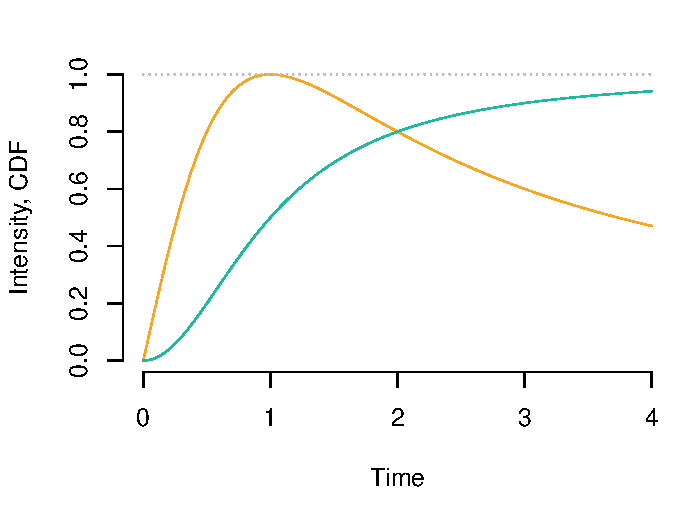
\includegraphics[width=\textwidth]{\FIGDIR/dwellDist01}
    \caption{$q(t) = \frac{2t}{t^2 + 1}$}
  \end{subfigure}
	\hfill
	\begin{subfigure}[b]{0.46\textwidth}
    \centering
		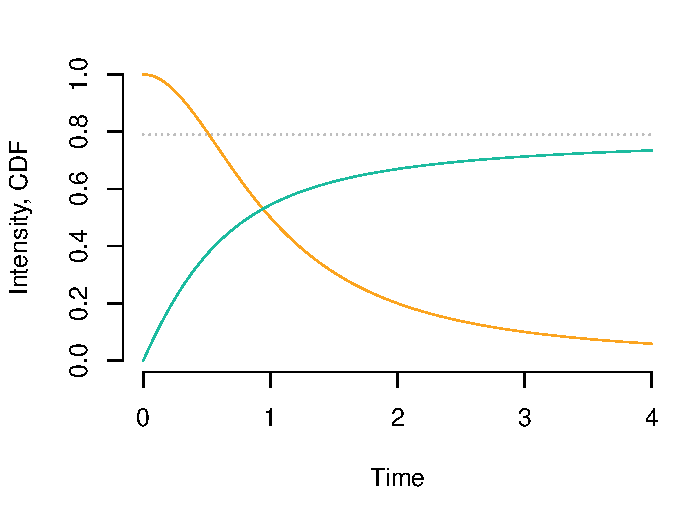
\includegraphics[width=\textwidth]{\FIGDIR/dwellDist02}
    \caption{$q(t) = \frac{1}{t^2 + 1}$}
  \end{subfigure}

	\begin{subfigure}[b]{0.46\textwidth}
    \centering
		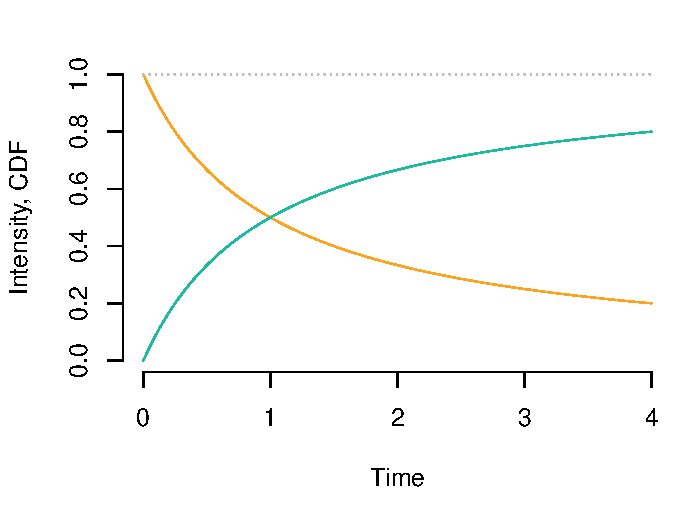
\includegraphics[width=\textwidth]{\FIGDIR/dwellDist03}
    \caption{$q(t) = \frac{1}{t + 1}$}
  \end{subfigure}
	\hfill
	\begin{subfigure}[b]{0.46\textwidth}
    \centering
		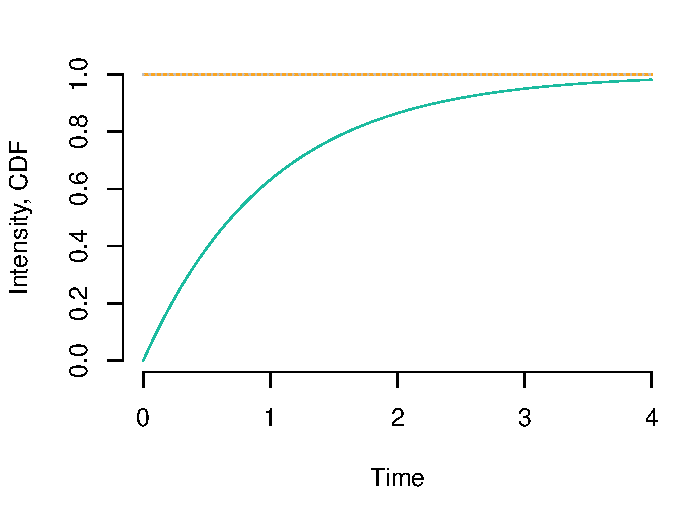
\includegraphics[width=\textwidth]{\FIGDIR/dwellDist04}
    \caption{$q(t) = 1$}
  \end{subfigure}

	\caption{Comparison of several transition rates (orange lines), their respective cumulative distribution functions of dwell time (blue lines), and limits of CDF (gray dashed lines. In the last plot we can see CDF of exponential distribution Exp(1).}
	\label{fig:dwellDist}
\end{figure}


\begin{proposition}
	Let random variable $\tau_{s,i}$ be the first time process leaves state $i$ after time $s \geq 0$ and $X_s = i$, i.e. the random variable defined in \eqref{eq:tausi}. The process first transitions into state $j$ with probability
	\begin{equation}
		\label{eq:transProb}
		\pr [X_{\tau_{s,i}} = j \vert X_s = i ] = \E \left[ \frac{q_{ij}(\tau_{s,i})}{q_i(\tau_{s,i})} \right].
	\end{equation}
\end{proposition}

\begin{proof}
	Denote $F_{\tau}$ the cumulative distribution function of random variable $\tau_{s,i}$ and recall the support of $\tau_{s,i}$ is interval $(s, \infty)$. Then, by applying continuous Bayes' formula, we get
	\begin{multline*}
		\pr [X_{\tau_{s,i}} = j \vert X_s = i ] 
		= \int_s^\infty \pr [X_{\tau_{s,i}} = j \vert X_s = i, \tau_{s,i} = t] dF_{\tau} (t) \\
		= \int_s^\infty \pr [X_{t} = j \vert X_{t} \neq j, X_r = i, s \leq r < t] dF_{\tau} (t)
		= \int_s^\infty \frac{q_{ij}(t)}{q_{i}(t)} dF_{\tau} (t)
		= \E \left[ \frac{q_{ij}(\tau_{s,i})}{q_i(\tau_{s,i})} \right].
	\end{multline*}
\end{proof}

Note that the transition probability \eqref{eq:transProb} from previous proposition can be rewritten using the density of dwell time as
\[
	\E \left[ \frac{q_{ij}(\tau_{s,i})}{q_i(\tau_{s,i})} \right] =
	\int_0^\infty \exp \left(- \int_{s}^{s+x} q_i(t) dt \right) q_{ij}(s+x) dx.
\]

\begin{definition}
	\label{def:embedded}
	Let $\procX$ be a Markov process with transition times $T_1, T_2, ...$. Then we call a sequence of random variables
	\[
		\{ Y_k = X_{T_k}, k \in \N_0 \}
	\]
	an \emph{embedded chain}.
\end{definition}

\cite{PraskovaLachout12} proved that embedded chain of homogeneous Markov process is homogeneous Markov chain.
It is clear that embedded chain of inhomogeneous Markov process is again inhomogeneous.
We can further show that the chain does not have Markov property.
Take, for example, intensity matrix
\[
	\m{Q} (t) = 
		\begin{pmatrix}
			- \lambda & 0             & \lambda     & 0 & 0 \\
			0         & - 1 / \lambda & 1 / \lambda & 0 & 0 \\
			0         & 0             & - \lambda   & \lambda \mathbb{I} [t \leq 1] & \lambda \mathbb{I} [t > 1] \\
			0         & 0             & 0           & -1 & 1 \\
			0         & 0             & 0           & 1 & -1 \\
		\end{pmatrix}
\]
and initial probability vector $\m{p} = (1/2, 1/2, 0, 0, 0)$ with state space $\S = \{1, ..., 5 \}$.
Then it holds for the embedded chain $\{Y_t, t \in \N_0 \}$
\begin{align*}
	\pr [ Y_3 = 4 \vert Y_2 = 3, Y_1 = 1] \to 1 \qquad \text{as} \qquad \lambda \to \infty \\
	\pr [ Y_3 = 4 \vert Y_2 = 3, Y_1 = 2] \to 0 \qquad \text{as} \qquad \lambda \to \infty
\end{align*}
Hence this chain does not have Markov property.
However, we are still able to derive its distribution.

\begin{corollary}
	Let Markov process $\procX$ enter the state $i$ at time $s$. Then the joint distribution of the dwell time and the new state has the density
	\[
		f_{s,i} (x, j) = \exp \left(- \int_{s}^{s+x} q_i(t) dt \right) q_{i,j}(s+x)
	\]
	with respect to product of Lebesgue measure on $(0, \infty)$ and counting measure on $\S \setminus \{i\}$.
\end{corollary}

\begin{proof}
	The joint density is a product of marginal density of dwell time (Proposition~\ref{prop:dwellTime}) and conditional transition probability (Proposition~\ref{prop:transProb})
\end{proof}



	
	
	




%%%%%%%%%%%%%%%%%%%%%%%%%%%%%%%%%%%%%%%%%%%%%%%%%%%%%%%%%%%%%%%%%%%%%%%%%%%%%%%%%%%%%%%
%%%%%%%%%%%%%%%%%%%%%%%%%%%%%%%%%%%%%%%%%%%%%%%%%%%%%%%%%%%%%%%%%%%%%%%%%%%%%%%%%%%%%%%
\section{Separable Inhomogeneity}
\label{chap:separable}

In this section, we will study family of inhomogeneous Markov processes for which transition rates vary over time in the same manner for each transition between pairs $i, j \in \S$, $i \neq j$.

\begin{definition}
	\label{def:separable}
	Let $\procX$ be inhomogeneous Markov process with transition matrix $\m{Q} (t)$. If there exists a function $\lambda: \Rplus \to (0, \infty)$ and a (constant-in-time) matrix $\m{\Gamma}$ such that
\[
	\m{Q}(t) = \lambda(t) \m{\Gamma}, \qquad \forall t \geq 0
\]
then we say that $\m{X}$ is Markov process with \emph{separable inhomogeneity}.

We will call $\lambda$ a \emph{separated inhomogeneity} and $\m{\Gamma}$ a \emph{constant rate matrix}.
\end{definition}

\begin{definition}
	\label{def:homoTrans}
	Suppose that $\procX$ is an inhomogeneous Markov process and $\m{Y} = \{Y_t, \, t \geq 0 \}$ is a homogeneous Markov process. We say that $\m{Y}$ is \emph{homogeneous transformation} of $\m{X}$ if there exists an increasing and differentiable function $\tau : \Rplus \to \Rplus$, $\tau (0) = 0$ such that $X_{\tau(t)} = Y_t$ a.s.
\end{definition}

Following theorem justifies the equivalency of previous definitions. The proof of the theorem provides a way how to construct the time-transformation function $\tau$ and separated intensity function $\lambda$.

\begin{proposition}
	\label{prop:separable}
	Markov process $\procX$ has separable inhomogeneity if and only if there exists a homogeneous transformation of $\m{X}$.
\end{proposition}

\begin{proof}
	Let $\m{X}$ has separable inhomogeneity with notation from Definition~\ref{def:separable}. Define $\m{Y}$ as $Y_t = X_{\tau(t)}$, where $\tau(t) = \Lambda^{-1} (t)$. Because the function $\tau$ is increasing, the Markov property holds for the process $\m{Y}$ as well. The transition probabilities of $\m{Y}$ are given by
	\begin{align*}
		p_{ij}^{(Y)} (t, t+h)
		=& \pr [ Y_{t+h} = j \vert Y_t = i ]
		= \pr [ X_{\tau (t+h)} = j \vert X_{\tau (t)} = i ] \\
		=& \gamma_{ij} \lambda(\tau (t)) \left( \Lambda^{-1} (t+h) - \Lambda^{-1} (t) \right) + o(h).
	\end{align*}
	The derivative of inverse function is given by
	\[
		\frac{\partial \Lambda^{-1} (t)}{\partial t} = \frac{1}{\lambda (\Lambda^{-1} (t))},
	\]
	which implies that the intensity of $\m{Y}$ is $q_{ij}^{(Y)} (t) = \gamma_{ij}$ and does not depend on time $t$.
	
	Suppose there exists a process $\m{Y}$ that is a homogeneous transformation of $\m{X}$ with time-transformation function $\tau$ as in Definition~\ref{def:homoTrans} and the intensity matrix of $\m{Y}$ is $\bm{\Gamma}$. The transition probabilities of $\m{X}$ are given by
		\begin{align*}
		p_{ij}^{(X)} (t, t+h)
		=& \pr [ X_{t+h} = j \vert X_t = i ]
		= \pr [ Y_{\tau^{-1} (t+h)} = j \vert Y_{\tau^{-1} (t)} = i ] \\
		=& \gamma_{ij} \left( \tau^{-1} (t+h) - \tau^{-1} (t) \right) + o(h).
	\end{align*}
	Therefore $\m{X}$ has separated inhomogeneity with constant rate matrix $\bm{\Gamma}$ and function
	\[
		\lambda(t) = \frac{\partial \tau^{-1} (t)}{\partial t}.
	\]

\end{proof}

In previous chapter we showed that embedded chain of inhomogeneous Markov process does not have to be Markov chain.
On the other hand, if the process has separable inhomogeneity its embedded chain is homogeneous Markov Chain.
That is because such process has homogeneous transformation by Proposition~\ref{prop:separable} and both the process and its homogeneous transformation have almost surely the same embedded chain.
This property is convenient, for example, when simulating such process.
One can simulate first the embedded chain and then the dwell times.

	
	




%%%%%%%%%%%%%%%%%%%%%%%%%%%%%%%%%%%%%%%%%%%%%%%%%%%%%%%%%%%%%%%%%%%%%%%%%%%%%%%%%%%%%%%
%%%%%%%%%%%%%%%%%%%%%%%%%%%%%%%%%%%%%%%%%%%%%%%%%%%%%%%%%%%%%%%%%%%%%%%%%%%%%%%%%%%%%%%
\section{Inhomogeneous Poisson Process}
\label{chap:poisson}

Poisson process is widely used as a counting process for number of events that occur independently over a time interval. In practice, we sometimes face problems that violate the assumptions of homogeneity of the process. In this section we introduce process that generalizes the definition of Poisson process. Let us begin with definition of inhomogeneous Poisson process.

\begin{definition}
	\label{def:inhomogeneousPoisson}
	Suppose that $N = \{N_t, t \geq 0\}$ is a counting process with values in $\N_0$ and $\lambda : \Rplus \to \Rplus$ be a real function. We call $N$ an \emph{inhomogeneous Poisson process} if it follows
	\begin{enumerate}[i)]
		\item $N_0 = 0$ a.s.;
		\item Increments of $N$ are independent;
		\item $\pr [ N_{t+h} = i+1 \vert N_t = i ] = \lambda(t) h + o(h)$;
		\item $\pr [ N_{t+h} > i+1 \vert N_t = i ] = o(h)$.
	\end{enumerate}
\end{definition}

Clearly, if $\lambda$ is constant, non-zero function then $N$ is homogeneous Poisson process. Inhomogeneous Poisson process is a special case of Markov process with separable inhomogeneity with transition rate matrix
\[
	\m{Q}(t) = \begin{pmatrix}
			-\lambda (t) & \lambda (t) & 0 & \cdots \\
			0 & -\lambda (t) & \lambda (t) &  \\
			\vdots & & \ddots & \ddots
\end{pmatrix} = \lambda (t) \begin{pmatrix}
			-1 & 1 & 0 & \cdots \\
			0 & -1 & 1 &  \\
			\vdots & & \ddots & \ddots
\end{pmatrix}.
\]

The distribution of Poisson process and its increments is again Poisson, i.e.
\begin{align*}
	N_t & \sim Poi (\Lambda(t)), \\
	N_s - N_t & \sim Poi (\Lambda(s) - \Lambda(t)),
\end{align*}
where $\Lambda(t) = \int_0^t \lambda(t) dt$.
The reader can find a proof for example in \cite{Lewis79}. Another way to show this is to use the fact that the inhomogeneous Poisson process is also an inhomogeneous Markov process with separable inhomogeneity. Then there exists by \nameref{prop:separable} a homogeneous transformation with unit intensity and transformation function $\tau (t) = \Lambda^{-1} (t)$. This can be used to simulate an inhomogeneous Poisson process on time interval $[0, T]$.

\begin{algorithm}[Simulating Poisson process]\
	\label{algo:simulPoisson}
	\begin{enumerate}
		\item Simulate number of transitions $N \sim Poi (\Lambda(T))$.
		\item Simulate independent random variables $R_i \sim Exp(1)$ for $i = 1, ..., N+1$.
		\item Calculate ordered transition times of the homogeneous transformation on interval $[0,1]$
			\[
				S_k = \frac{\sum_{i=1}^{k} R_i}{\sum_{i=1}^{N+1} R_i}, \qquad k = 1, ..., N.
			\]
		\item Transform to transition times of the inhomogeneous Poisson process
			\[
				T_k = \Lambda^{-1} (S_k \times \Lambda(T)), \qquad k = 1, ..., N,
			\]
		\item Return the transition times $T_1, ..., T_N$.
	\end{enumerate}
\end{algorithm}



Denote by $T_1, T_2, ...$ the increasing sequence of (random) jump times of inhomogeneous Poisson process. Their distributions are given by Proposition \ref{prop:dwellTime}. Let $Z_1, Z_2, ...$ be a sequence of independent random variables with distribution measures $\mu_{T_i}$. Then we can define random process $\m{M} = \{ M-t, t \geq 0 \}$ by
\[
	M_t = \sum_{i=1}^{\infty} Z_i \times \mathbb{I} [t \geq T_i].
\]
Let us call this process an \emph{inhomogeneous compound Poisson process}. In following Proposition we show the property of such process if the distributions of $Z_i$ are Bernoulli.

\begin{proposition}
	\label{prop:compoundPoisson}
	Let $N = \{N_t, t \geq 0\}$ be an inhomogeneous Poisson process with intensity $\lambda(t)$ and jump times $T_1, T_2, ...$. Let $\pi: \Rplus \to (0,1)$ be a right-continuous function and $Z_i \sim Alt(\pi(T_i))$. Then the family of random variables
	\[
		M_t = \sum_{i=1}^{\infty} Z_i \times \mathbb{I} [t \geq T_i].
	\]
	is an inhomogeneous Poisson process with intensity $\lambda(t) \pi(t)$.
\end{proposition}

\begin{proof}
	Since $M$ is non-negative process and $M_t \leq N_t$ a.s. for any $t \geq 0$, then also $M_0 = 0$ a.s. The increments of $N$ are independent by definition and also the values of $Z_i$ are mutually independent. Therefore the increments of $M$ are also independent.
	
	Because the function $\pi$ is right continuous, one can write $\pi(t+h) = \pi(t) + o(h)$. The probability of jump in a small interval is bounded by
	\begin{align*}
		\pr [ M_{t+h} = j+1 \vert M_t = j ]
		&\geq \pr [ N_{t+h} = i+1 \vert N_t = i ] \times (\pi(t) + o(h)) \\
		&= (\lambda(t) h + o(h)) \times (\pi(t) + o(h)) = \lambda(t)\pi(t) h + o(h)\\
	\end{align*}
	and
	\begin{align*}
		\pr [ M_{t+h} = j+1 \vert M_t = j ]
		&\leq \lambda(t)\pi(t) h + o(h) + \pr [ N_{t+h} > i+1 \vert N_t = i ] \\
		&= \lambda(t)\pi(t) h + o(h),
	\end{align*}
	Which implies that the probability is equal to both the boundaries. Also
	\[
		\pr [ M_{t+h} > j+1 \vert M_t = j ] \leq \pr [ N_{t+h} > i+1 \vert N_t = i ]
	\]
	implies point \emph{iv} in Definition~\ref{def:inhomogeneousPoisson}.
\end{proof}